% ============= setup ============= %
% ======== package ======== %
\documentclass[mathserif]{beamer}
\usepackage{xeCJK}
\usepackage{graphicx}
\usepackage{xcolor}
\usepackage{setspace}
\usepackage{newtxmath}

% ======== font ======== %
\setCJKmainfont{Taipei Sans TC Beta}
\setCJKsansfont{Taipei Sans TC Beta}
\AtBeginDocument{%
    \DeclareSymbolFont{pureletters}{OML}{cmm}{m}{it}%
    \SetSymbolFont{pureletters}{bold}{OML}{cmm}{b}{it}%
}
\hypersetup{
    colorlinks=true,
    linkcolor=black,
    urlcolor=blue
}

% ======== theme ======== %
\renewcommand{\baselinestretch}{1.25}
\usetheme{Madrid}
\usecolortheme{crane}
\setbeamertemplate{items}[circle]
\setbeamertemplate{section in toc}{\inserttocsectionnumber.~\inserttocsection}
\AtBeginSection[]{
    \begin{frame}
        \vfill
        \centering
        \begin{beamercolorbox}[sep=8pt,center,shadow=true,rounded=true]{title}
            \usebeamerfont{title}\insertsectionhead\par%
        \end{beamercolorbox}
        \vfill
    \end{frame}
}

% ======== data ======== %
\title{二分搜尋}
\author{temmie}
\date{}

% ============= setup ============= %

\begin{document}

\begin{frame}
    \titlepage
\end{frame}

\begin{frame}
    \tableofcontents
\end{frame}

\section{二分搜簡介}

\begin{frame}
    \frametitle{二分搜簡介}
    \begin{itemize}
        \item 讓我們試試看玩終極密碼\ :D
        \item<2-> 事實上,我們就是在做\textbf{搜尋答案}這件事情
        \item<2-> 我們總共搜尋了多少次?這樣的時間複雜度是多少呢?
    \end{itemize}
\end{frame}

\begin{frame}
    \frametitle{二分搜方法}
    \begin{itemize}
        \item 既然答案有可能在任何地方,那就中間切一刀吧!
        \item 這樣一定是最好,因為兩邊的機率都會是一半
        \item<2-> 二分搜就是\textbf{將資料切半,看答案在哪一邊}
        \item<2-> 時間複雜度是 $O(log_2\ n)$ ,因為每次資料量都會減少一半
    \end{itemize}

\end{frame}

\section{二分搜實作}

\begin{frame}
    \frametitle{結論}
    \begin{itemize}
        \item 我們會將陣列轉換成 01 陣列
        \item 如果尋找到的元素是 0 就做 A,否則做 B
        \item 如果沒辦法轉換成 01 陣列 = 沒有單調性 = 沒辦法二分搜
        \vspace{0.5cm}
        \item<2-> 二分搜的實作有很多方式,我會介紹我最常用的方式
        \item<2-> 實作有太多細節了,練習是唯一熟悉的方法
    \end{itemize}
\end{frame}

\begin{frame}
    \frametitle{實作:架構}
    \begin{itemize}
        \item 架構只會有兩點:二分搜主程式、判斷合法函式
        \item<2-> 前者不難,通常或寫得像模板一樣
        \item<2-> 後者通常較難,也就是題目想要你要思考\textbf{搜尋什麼}的地方。
    \end{itemize}
\end{frame}

\begin{frame}
    \frametitle{實作:二分搜主程式}
    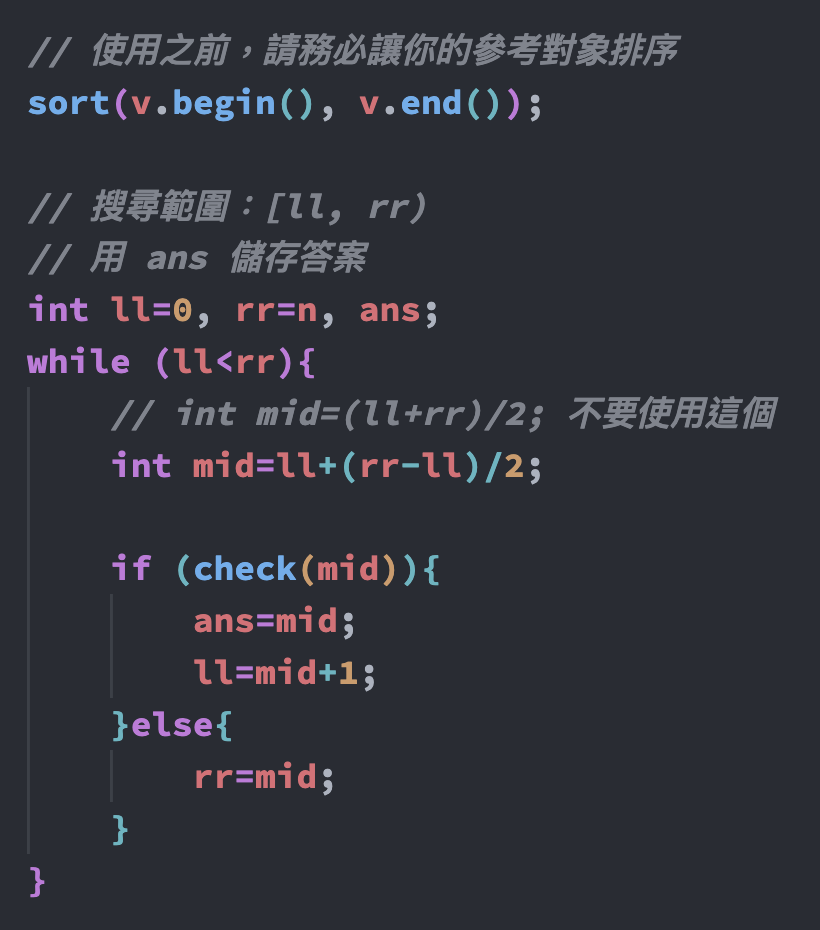
\includegraphics[width=7.0cm]{img/bs-main.png}
\end{frame}

\begin{frame}
    \frametitle{實作:判斷合法函式}
    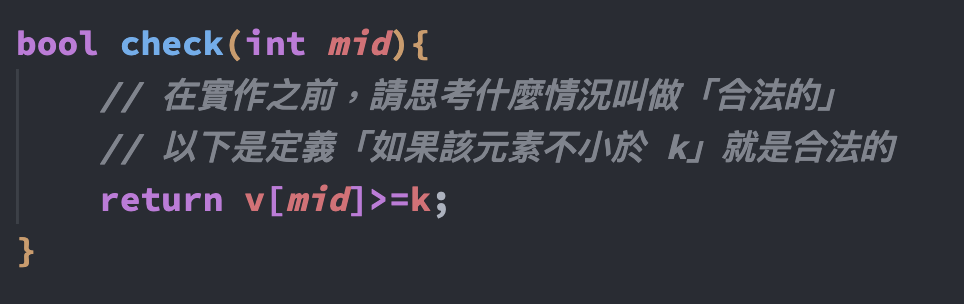
\includegraphics[width=11.0cm]{img/bs-check.png}
\end{frame}

\begin{frame}
    \frametitle{實作:常見 bug}
    \begin{itemize}
        \item 忘記排序
        \item 搜尋區間錯誤
        \item 計算 mid 的時候 overflow
    \end{itemize}
\end{frame}

\section{二分搜工具}

\begin{frame}
    \frametitle{簡介}
    \begin{itemize}
        \item STL 內建了很多好用的工具可以讓我們不用手刻二分搜
        \item 這類型的工具只適合在容器中使用
        \item 請注意:不要過度依賴工具,有很多題目是\textbf{只能手刻二分搜的}
    \end{itemize}
\end{frame}

\begin{frame}
    \frametitle{binary\_search}
    \begin{itemize}
        \item binary\_search({\color{red}L}, {\color{red}R}, {\color{red}val})
        \item 判斷 val 是否在 $[L, R)$ 裡面
    \end{itemize}
\end{frame}

\begin{frame}
    \frametitle{lower\_bound}
    \begin{itemize}
        \item lower\_bound({\color{red}L}, {\color{red}R}, {\color{red}val})
        \item 回傳 $[L, R)$ 中最左 $\geq val$ 的值迭代器位置
        \item<2-> 如果想要得到該值需要使用\ {\color{red}*}lower\_bound(L, R, val)
        \item<2-> 如果想要得到該值的索引值需要使用\ {\color{red}*}lower\_bound(L, R, val){\color{red}-L}
    \end{itemize}
\end{frame}

\begin{frame}
    \frametitle{upper\_bound}
    \begin{itemize}
        \item upper\_bound({\color{red}L}, {\color{red}R}, {\color{red}val})
        \item 回傳 $[L, R)$ 中最左 $> val$ 的值迭代器位置
        \item<2-> 如果想要得到該值需要使用\ {\color{red}*}upper\_bound(L, R, val)
        \item<2-> 如果想要得到該值的索引值需要使用\ {\color{red}*}upper\_bound(L, R, val){\color{red}-L}
    \end{itemize}
\end{frame}

\begin{frame}
    \frametitle{例題}
    \begin{block}{例題}
        \begin{itemize}
            \item \href{https://codeforces.com/edu/course/2/lesson/6/1/practice/contest/283911/problem/A}{搜尋元素}
            \item \href{https://codeforces.com/edu/course/2/lesson/6/1/practice/contest/283911/problem/B}{不大於 k 的數}
            \item \href{https://codeforces.com/edu/course/2/lesson/6/1/practice/contest/283911/problem/C}{不小於 k 的數}
            \item \href{https://codeforces.com/edu/course/2/lesson/6/1/practice/contest/283911/problem/D}{區間數值數量}
        \end{itemize}

        上面的例題請用二分搜工具思考,回家後記得手刻一次寫法!
    \end{block}
\end{frame}

\section{對答案二分搜}

\begin{frame}
    \frametitle{簡介}
    \begin{itemize}
        \item 上一個章節裡面我們都是提到在容器裡二分搜
        \item 在這裡,提供一個新的思路叫做\textbf{對答案二分搜}
    \end{itemize}
\end{frame}

\begin{frame}
    \frametitle{例題}
    \begin{block}{例題}
        \begin{itemize}
            \item \href{https://codeforces.com/edu/course/2/lesson/6/2/practice/contest/283932/problem/A}{貨物包裝}
            \item \href{https://cses.fi/problemset/task/1620}{機器排程}
        \end{itemize}

        上面的例題中,會發現我們不是再那麼「無腦的」寫判斷合法函式,\\
        通常會帶有更多的思考。
    \end{block}
\end{frame}

\section{對第 $k$ 大二分搜}

\begin{frame}
    \frametitle{簡介}
    \begin{itemize}
        \item 這個章節是一個比較特殊的二分搜
        \item 如果題目有單調性並且提到第 $k$ 大/小,那就很有機會是二分搜
        \item 需要能夠計算該值是是第幾大/小
    \end{itemize}
\end{frame}

\begin{frame}
    \frametitle{例題}
    \begin{block}{例題}
        \begin{itemize}
            \item \href{https://cses.fi/problemset/task/2422}{乘法表}
            \item \href{https://codeforces.com/edu/course/2/lesson/6/5/practice/contest/285084/problem/C}{第 $k$ 小數對和}
        \end{itemize}
    \end{block}
\end{frame}

\end{document}